% !TeX root = Stageportfolio.tex



\begin{landscape}
	\subsubsection{Les 16}
	\begin{tabularx}{1.56\textwidth}{|p{0.35\textwidth}|X|}\hline
		\textbf{Administratieve gegevens}\newline\newline
		Kevin Truyaert\newline\newline
		technisch secundair onderwijs\newline
		3e graad, 1ste jaar, Techniek-Wetenschappen\newline
		VVKSO: \href{http://ond.vvkso-ict.com/leerplannen/doc/Toegepaste\%20fysica-2014-041.pdf}{http://ond.vvkso-ict.com/leerplannen /doc/Toegepaste\%20fysica-2014-041.pdf} \newline
		\underline{Lesonderwerp}:\newline Wet van Lenz \& algemene inductiewet: Faraday-Lenz + oefeningen & \textbf{Doelstellingen}
		\begin{itemize}[itemsep=0.08\baselineskip]
			\item B27: Fluxverandering als oorzaak van inductiespanning toelichten
			\item B28: Met behulp van de wet van Lenz de zin van de inductiespanning vinden
			\item B29: De algemene inductiewet hanteren.
		\end{itemize}
		\underline{Lesdoelen}\newline
		\vspace{-0.75cm}
		\begin{enumerate}[itemsep=0.08\baselineskip]
			\item De leerlingen kunnen de zin van de inductiestroom bepalen.
			\item De leerlingen kunnen de wet van Lenz verwoorden.
			\item De leerlingen zien de samenhang tussen de wet van Faraday en de wet van Lenz in.
			\item De leerlingen kennen de wet van Faraday-Lenz.
			\item De leerlingen kunnen de wet van Faraday-Lenz op een rechte, bewegende geleider toepassen.
			\item De leerlingen kennen de relatie tussen inductiespanning, magnetisch veld, lengte van de geleider, snelheid van de geleider en aantal windingen.
			\item De leerlingen kunnen de algemene inductiewet tijdens oefeningen hanteren.
		\end{enumerate} \\\hline
	\end{tabularx}\vfill \textcolor{white}{.} 


	\begin{tabularx}{1.56\textwidth}{|p{0.55\textwidth}|X|}
		\hline
		\multirow{2}{0.55\textwidth}{\textbf{Beginsituatie}\newline  
		Er zijn acht leerlingen binnen 5TW. Er heerst een algemene klassfeer. De leerlingen hebben al theorie gekregen  rond en oefeningen gemaakt op de magnetische krachtwerking. \newline\newline De leerlingen hebben vorige week de wet van Faraday gezien. Hiermee kunnen ze de grootte van de inductiespanning bepalen. Ook met de begrippen flux en fluxverandering zijn ze gekend. \newline\newline NOG AANVULLEN MET LERAARKENMERKEN.} & \textbf{Acties}\newline\newline %Vandaag worden de belangrijkste aspecten hiervan nog even overlopen. Daarnaast zijn we gisteren ook begonnen aan een nieuw stuk theorie rond elektromagnetische inductie. Hiervan hebben we de basis rond magnetische flux al besproken. Dit wordt nog even terug aangehaald.
		- \GreenHighlight{Via demo's wil ik bepaalde onderwerpen starten.}{9cm}	Op die manier kan ik de interesse van de leerlingen wekken en kan ik fysische wetmatigheden hen effectief aantonen. Zo kunnen leerlingen op een klassikale manier zelfstandig dingen ontdekken.	 \newline\newline 
		- Ik wil oefeningen op zo'n wijze brengen dat ze steeds dezelfde structuur hebben. Die structuur bouw ik eerst samen met de leerlingen op, om ze daarna zelfstandig aan de slag te laten gaan met oefeningen die steeds wat complexer worden. \PinkHighlight{Tijdens het zelfstandig maken van de oefeningen probeer ik toch zeker}{13cm} \PinkHighlight{de zwakkere leerlingen in de gaten te houden en hen individueler te coachen bij het}{15cm} \PinkHighlight{maken van oefeningen.}{5cm}
		\newline\newline\newline\newline\newline\newline
		
		\\ \cline{2-2}
		  & \textbf{Bronnen}\begin{itemize}
		  	\item Schramme, S. (2018) De stroombalans, labo magnetisme 4
		  	\item Frederiksen (2014), Current Balance 4565.00
		  	\item Giancoli, D. C. (2008). Physics for scientists and engineers. Pearson Education International.
		  \end{itemize}\\ \hline
	\end{tabularx}


\newpage
	
	\begin{tabularx}{1.56\textwidth}{|p{1.5cm}|p{9cm}|X|p{4cm}|}
		\hline
		\textbf{Nr. lesdoel } & \textbf{Inhoud (timing)}  & \textbf{Organisatie } & \textbf{Media } \\ \hline
		1	&\underline{Bespreking Labo M4:} \underline{de stroombalans (15 minuten)}\newline
		We gaan nog even dieper in op de effecten van de Lorentzkracht op de draad en de reactiekracht op de magneet om duidelijk te verklaren waarom de balans verschillen kon opmeten.
		&  \underline{Onderwijsleergesprek}\newline 
		De leerlingen krijgen hun door mij verbeterde labobundel terug en we overlopen de onderzoeksvragen van het labo nog even gezamenlijk. Ik vraag aan de leerlingen wat zij als essentie van het labo ervaren hebben. Vanuit dat standpunt wordt het labo besproken. Hierna wordt er niet meer terug gekomen op dit labo. Een duidelijk begrip van de Lorentzkracht is nodig voor de laatste twee hoofdstukken van magnetisme.
		&  Labobundel\newline\newline Slides (zie bijlage)
		\\ \hline
	\end{tabularx}\vspace{5mm}

	
\begin{tabularx}{1.56\textwidth}{|p{1.5cm}|p{8cm}|X|p{4cm}|}
	\hline
	\textbf{Nr. lesdoel } & \textbf{Inhoud (timing)}  & \textbf{Organisatie } & \textbf{Media } \\ \hline
	3\newline\newline 4\newline\newline &\underline{De algemene inductiewet:} \underline{Faraday-Lenz (10 minuten)}\newline
	We kunnen de wet van Faraday-Lenz besluiten als combinatie van de wet van Faraday en de wet van Lenz.
	&  \underline{Onderwijsleergesprek}\newline 
	De algemene inductiewet schrijf ik nu op bord. Ik vraag aan de leerlingen om ieder deel te verklaren.
	&   Cursus hoofdstuk 5 p13\newline\newline Krijtbord 
	\\ \hline
\end{tabularx}\vspace{5mm}


\begin{tabularx}{1.56\textwidth}{|p{1.5cm}|p{8cm}|X|p{4cm}|}
	\hline
	\textbf{Nr. lesdoel } & \textbf{Inhoud (timing)}  & \textbf{Organisatie } & \textbf{Media } \\ \hline
	5\newline\newline 6&\underline{Faraday-Lenz op een rechte, bewegende} \underline{geleider (5 minuten)}\newline
	Toepassen van Faraday-Lenz op een bewegende geleider.
	&  \underline{Onderwijsleergesprek}\newline 
	Ik schets de situatie van een bewegende, rechte geleider die aan spanningsmeter verbonden is. We leiden de spanning die door de beweging geïnduceerd is af, door middel van de gekende formules. Ik laat de leerlingen hier zelfstandig mee starten, gezien de verschillende stappen al op hun blad aanwezig zijn, waarna ik inpik.
	&   Cursus hoofdstuk 5 p13\newline\newline Krijtbord 
	\\ \hline
\end{tabularx}\vspace{5mm}



\begin{tabularx}{1.56\textwidth}{|p{1.5cm}|p{8cm}|X|p{4cm}|}
	\hline
	\textbf{Nr. lesdoel } & \textbf{Inhoud (timing)}  & \textbf{Organisatie } & \textbf{Media } \\ \hline
    1\newline\newline 4 \newline\newline 7& \underline{Faraday-Lenz: oefeningen (18 minuten)}\newline
    De leerlingen maken oefeningen op Faraday-Lenz.	
	&  \underline{Oefeningen + onderwijsleergesprek}\newline 
	Ik vraag aan de leerlingen om zelf even oefening 1 te maken. Hiervoor moeten ze gebruik maken van de wet van Lenz. Ik treed na een minuut in interactie met de leerlingen om mij het antwoord op de vragen te geven. Daarna maak ik, door middel van vraagstelling aan de leerlingen, oefening 2. Ik bouw alle stappen op die ze bij dit soort oefeningen zullen moeten doen. Daarna maken ze zelf oefeningen 3, 4 en 5.
	&  Cursus hoofdstuk 5 p14-15\newline\newline Krijtbord
	\\ \hline
\end{tabularx}\vspace{5mm}


\begin{tabularx}{1.56\textwidth}{|p{1.5cm}|p{8cm}|X|p{4cm}|}
	\hline
	\textbf{Nr. lesdoel } & \textbf{Inhoud (timing)}  & \textbf{Organisatie } & \textbf{Media } \\ \hline
	& \underline{Slot (2 minuten)}\newline
	Ik herhaal nog even kort de wet van Lenz en de algemene inductiewet. Deze zullen belangrijk zijn bij volgende lessen gezien die nog meer oefeningen hierover bevatten en er ook toepassingen van magnetische inductie besproken zullen worden.	
	&  \underline{Onderwijsleergesprek + vertellen}\newline 
	&  Cursus hoofdstuk 5 \newline\newline Krijtbord
	\\ \hline
\end{tabularx}

	
\end{landscape}


%\subsection*{Bijlage 5.1: slides introductie}

%
%\subsection*{Bijlage 1.2: bordschema theorie}
%\begin{center}
%	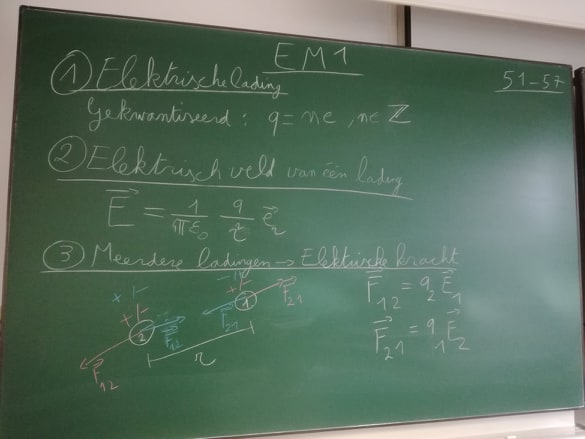
\includegraphics[width=0.9\textwidth]{Bord1a}
%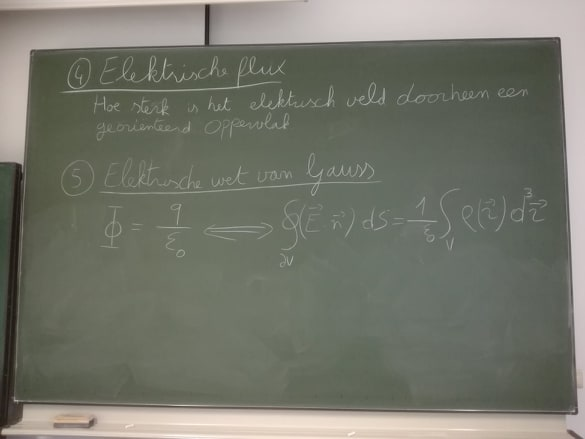
\includegraphics[width=0.9\textwidth]{Bord1b}
%\end{center}
%\newpage
%
%
%\includepdf[scale = 0.8,pages = 17,pagecommand=\subsection*{Bijlage 1.3: opgeloste oefeningen}]{Observaties_OpgelosteOef}
%\includepdf[scale = 0.8,pages =18-20,pagecommand=]{Observaties_OpgelosteOef}
%
%
%
%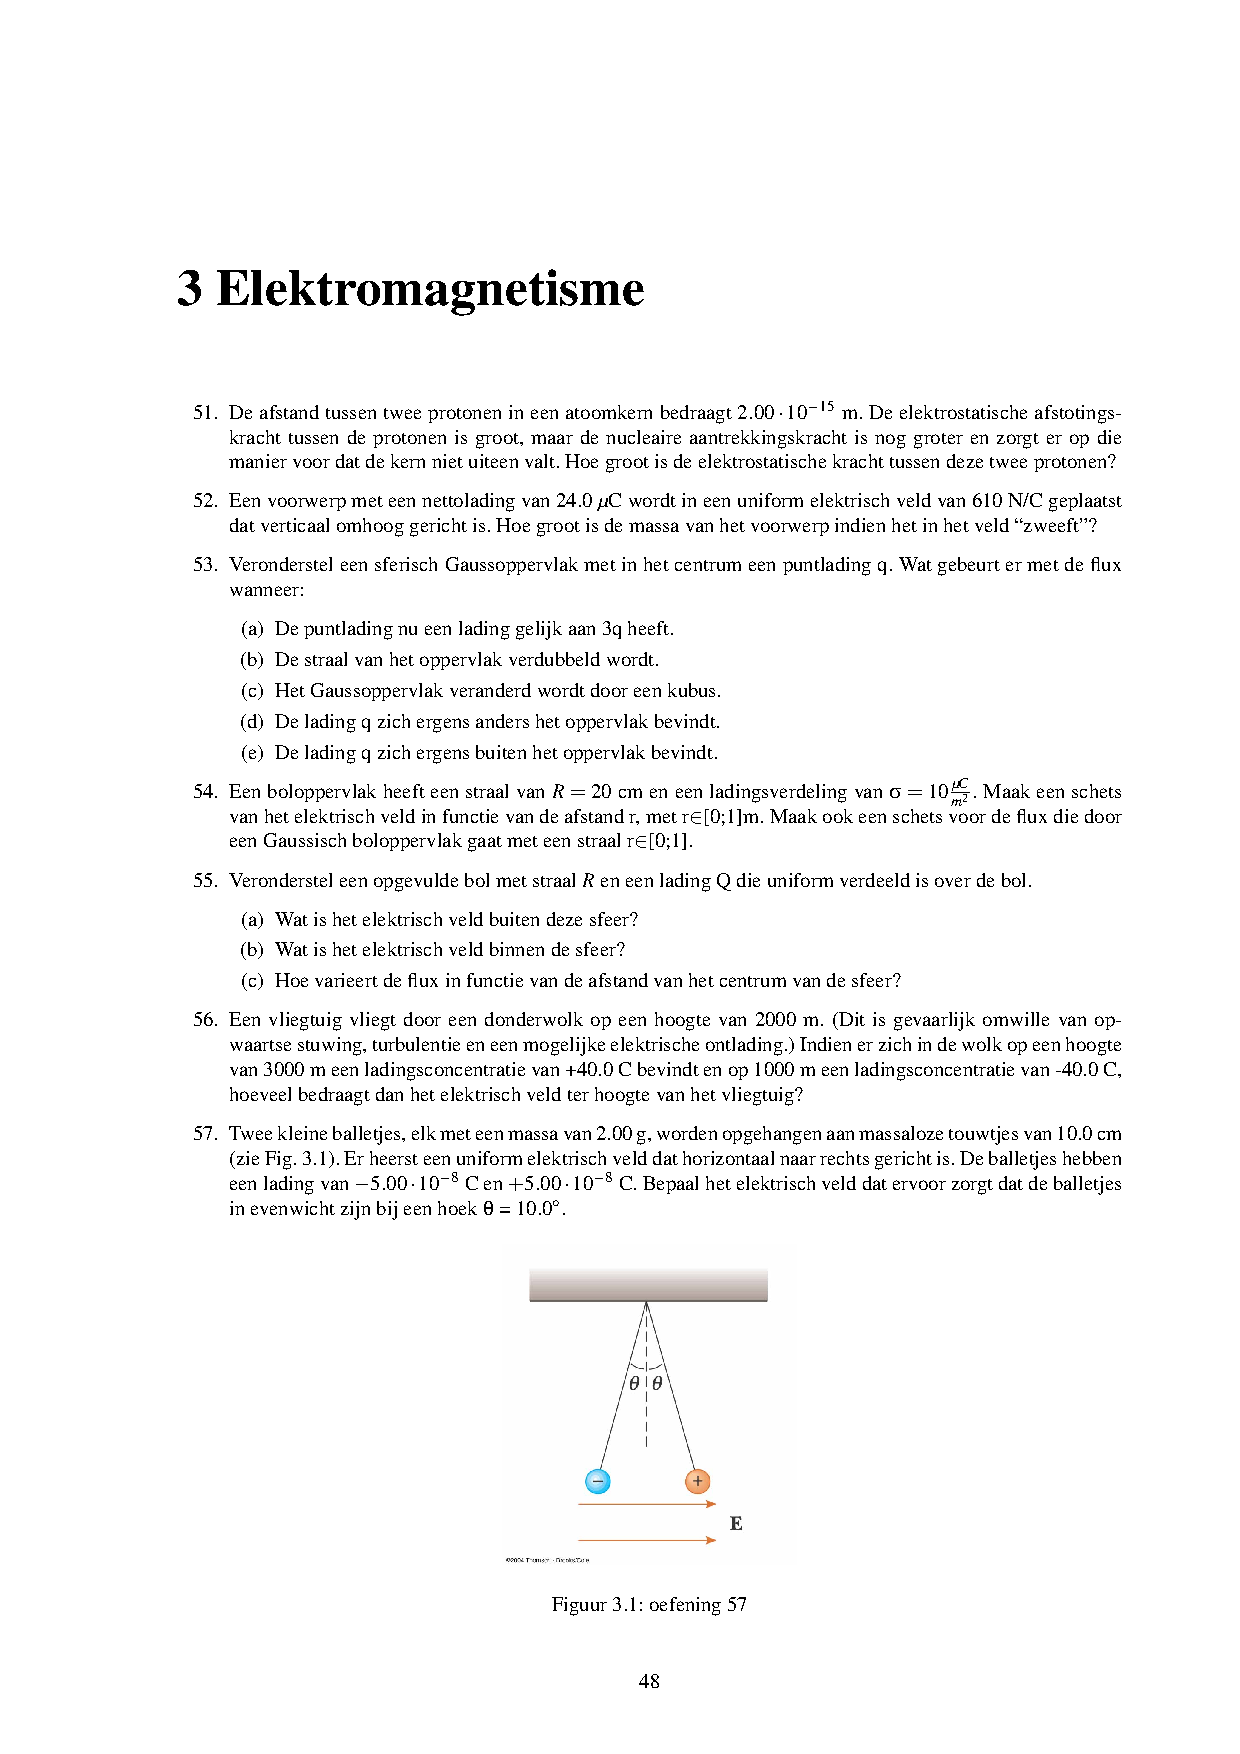
\includepdf[scale = 0.95,pages = 1,pagecommand=\subsection*{Bijlage 1.4: oefeningenbundel elektromagnetisme}]{OefeningenBundel}
%\includepdf[scale = 0.95,pages =2-,pagecommand=]{OefeningenBundel}